\chapter{Introduction to FPGA System}

\begin{figure}[H]
\centering
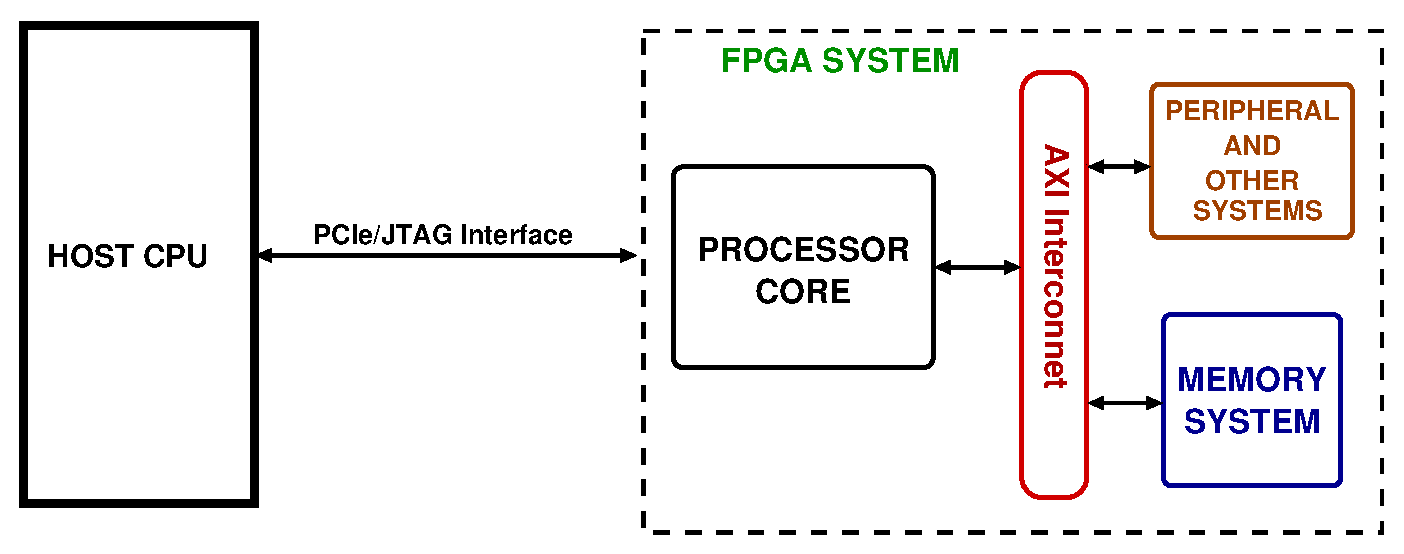
\includegraphics[width=\textwidth]{eps_pdf_sources/ajit_fpga/System_overview/fpga_system_intro}
\caption{Introduction to the FPGA System}
\end{figure}

The previous block diagram showed a telescopic view of the mentioned FPGA system. Now we expand a bit on the FPGA System block mentioned in
the previous diagram.

Here we introduce a generic interface architecture for building a system. As shown in the figure above the generic interface diagram of the
fpga model. Every subsystem including the processor core hanging from the interconnect appear just like a memory mapped peripheral to it.
This kind of architecture as explained at last in future work would provide a relatively easy extension to a Multiprocessor SMP model as
compared to a processor centric model. Some peripherals would act as AXI Slaves and some as AXI Masters depending on their functionality.
Another advantage to this architecture is that since each peripheral is memory mapped and JTAG has a direct access to the Interconnect one
can probe and read-write from-to any peripheral independent of the processor. As shown later after interfacing the PCIe to AXI we get
another possible data flow channel other than the standard UART and JTAG.  The number of peripherals that can be interfaced in this fashion
is only limited by the number of bits used for addressing on the interconnect.

\begin{figure}[H]
\centering
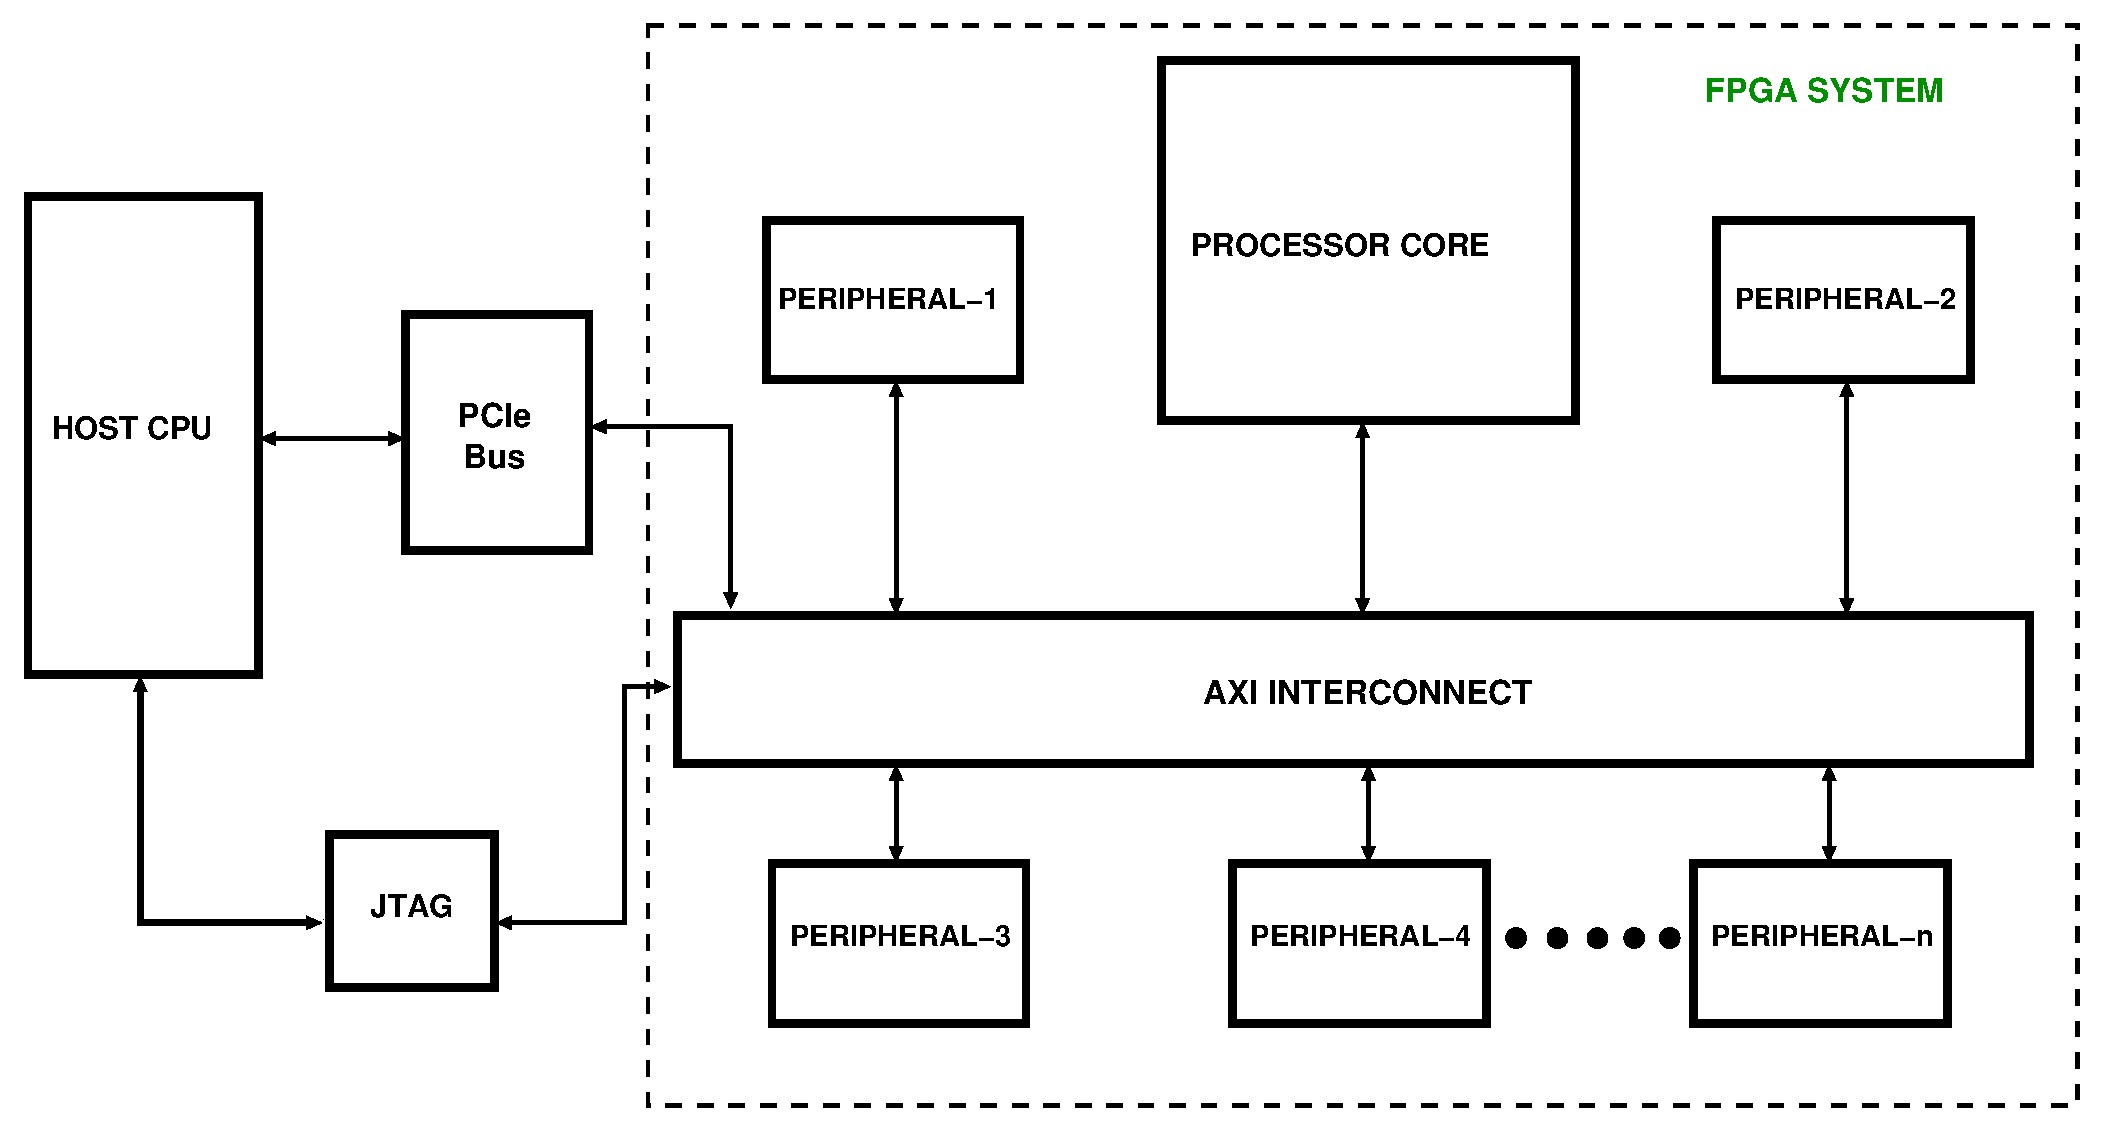
\includegraphics[width=\textwidth]{eps_pdf_sources/ajit_fpga/System_overview/fpga_system_expanded}
\caption{FPGA System Expanded}
\end{figure}
